% SLIDE
\begin{frame}
	\frametitle{The arms race}
	\begin{itemize}
		\item Ring 0 anti-cheat forces cheat developers to match that privilege level: does not solve the problem, only moves it
		\item BYOVD: exploiting legitimate signed drivers to inject malicious code
		\item Asymmetry: anti-cheat needs rigorous validation to ship, evasion techniques ship in days
		\item[$\Rightarrow$] A race the defender cannot win
	\end{itemize}
\end{frame}

% SLIDE
\begin{frame}
	\frametitle{The hardware blind spot}
	\begin{itemize}
		\item DMA cheats: a PCIe card reads host RAM directly, at the hardware layer
		\item Processing offloaded to a second PC — nothing runs on the gaming machine
		\item No driver, no process, no software footprint $\Rightarrow$ invisible to Ring 0 anti-cheat
	\end{itemize}
	\begin{center}
		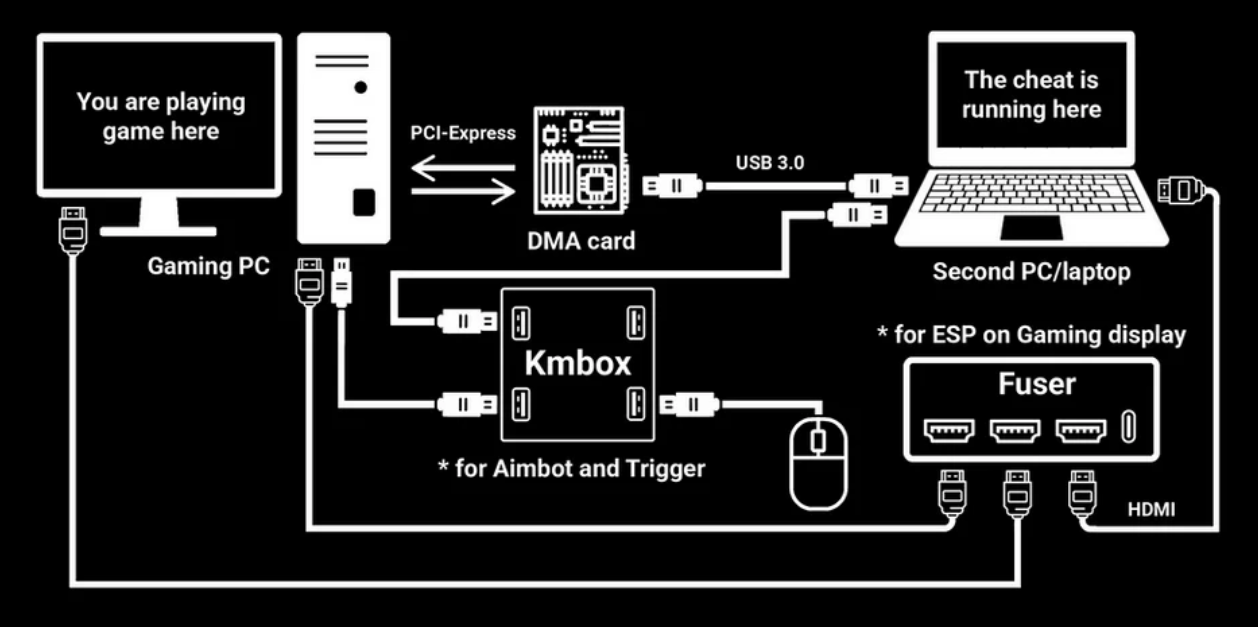
\includegraphics[height=4cm]{../images/chap01/fig5.png}
	\end{center}
\end{frame}

% SLIDE
\begin{frame}
	\frametitle{Experimental demonstration}
	\begin{itemize}
		\item Setup: isolated Windows 10 VM, Notepad seeded with a password, Windows-Kernel-Explorer + Cheat Engine
		\item Result: password located and reconstructed from RAM in minutes, with zero cooperation from the target process
		\item[$\Rightarrow$] Same inspection power a Ring 0 driver already has, by design, over every background process
	\end{itemize}
	\begin{center}
		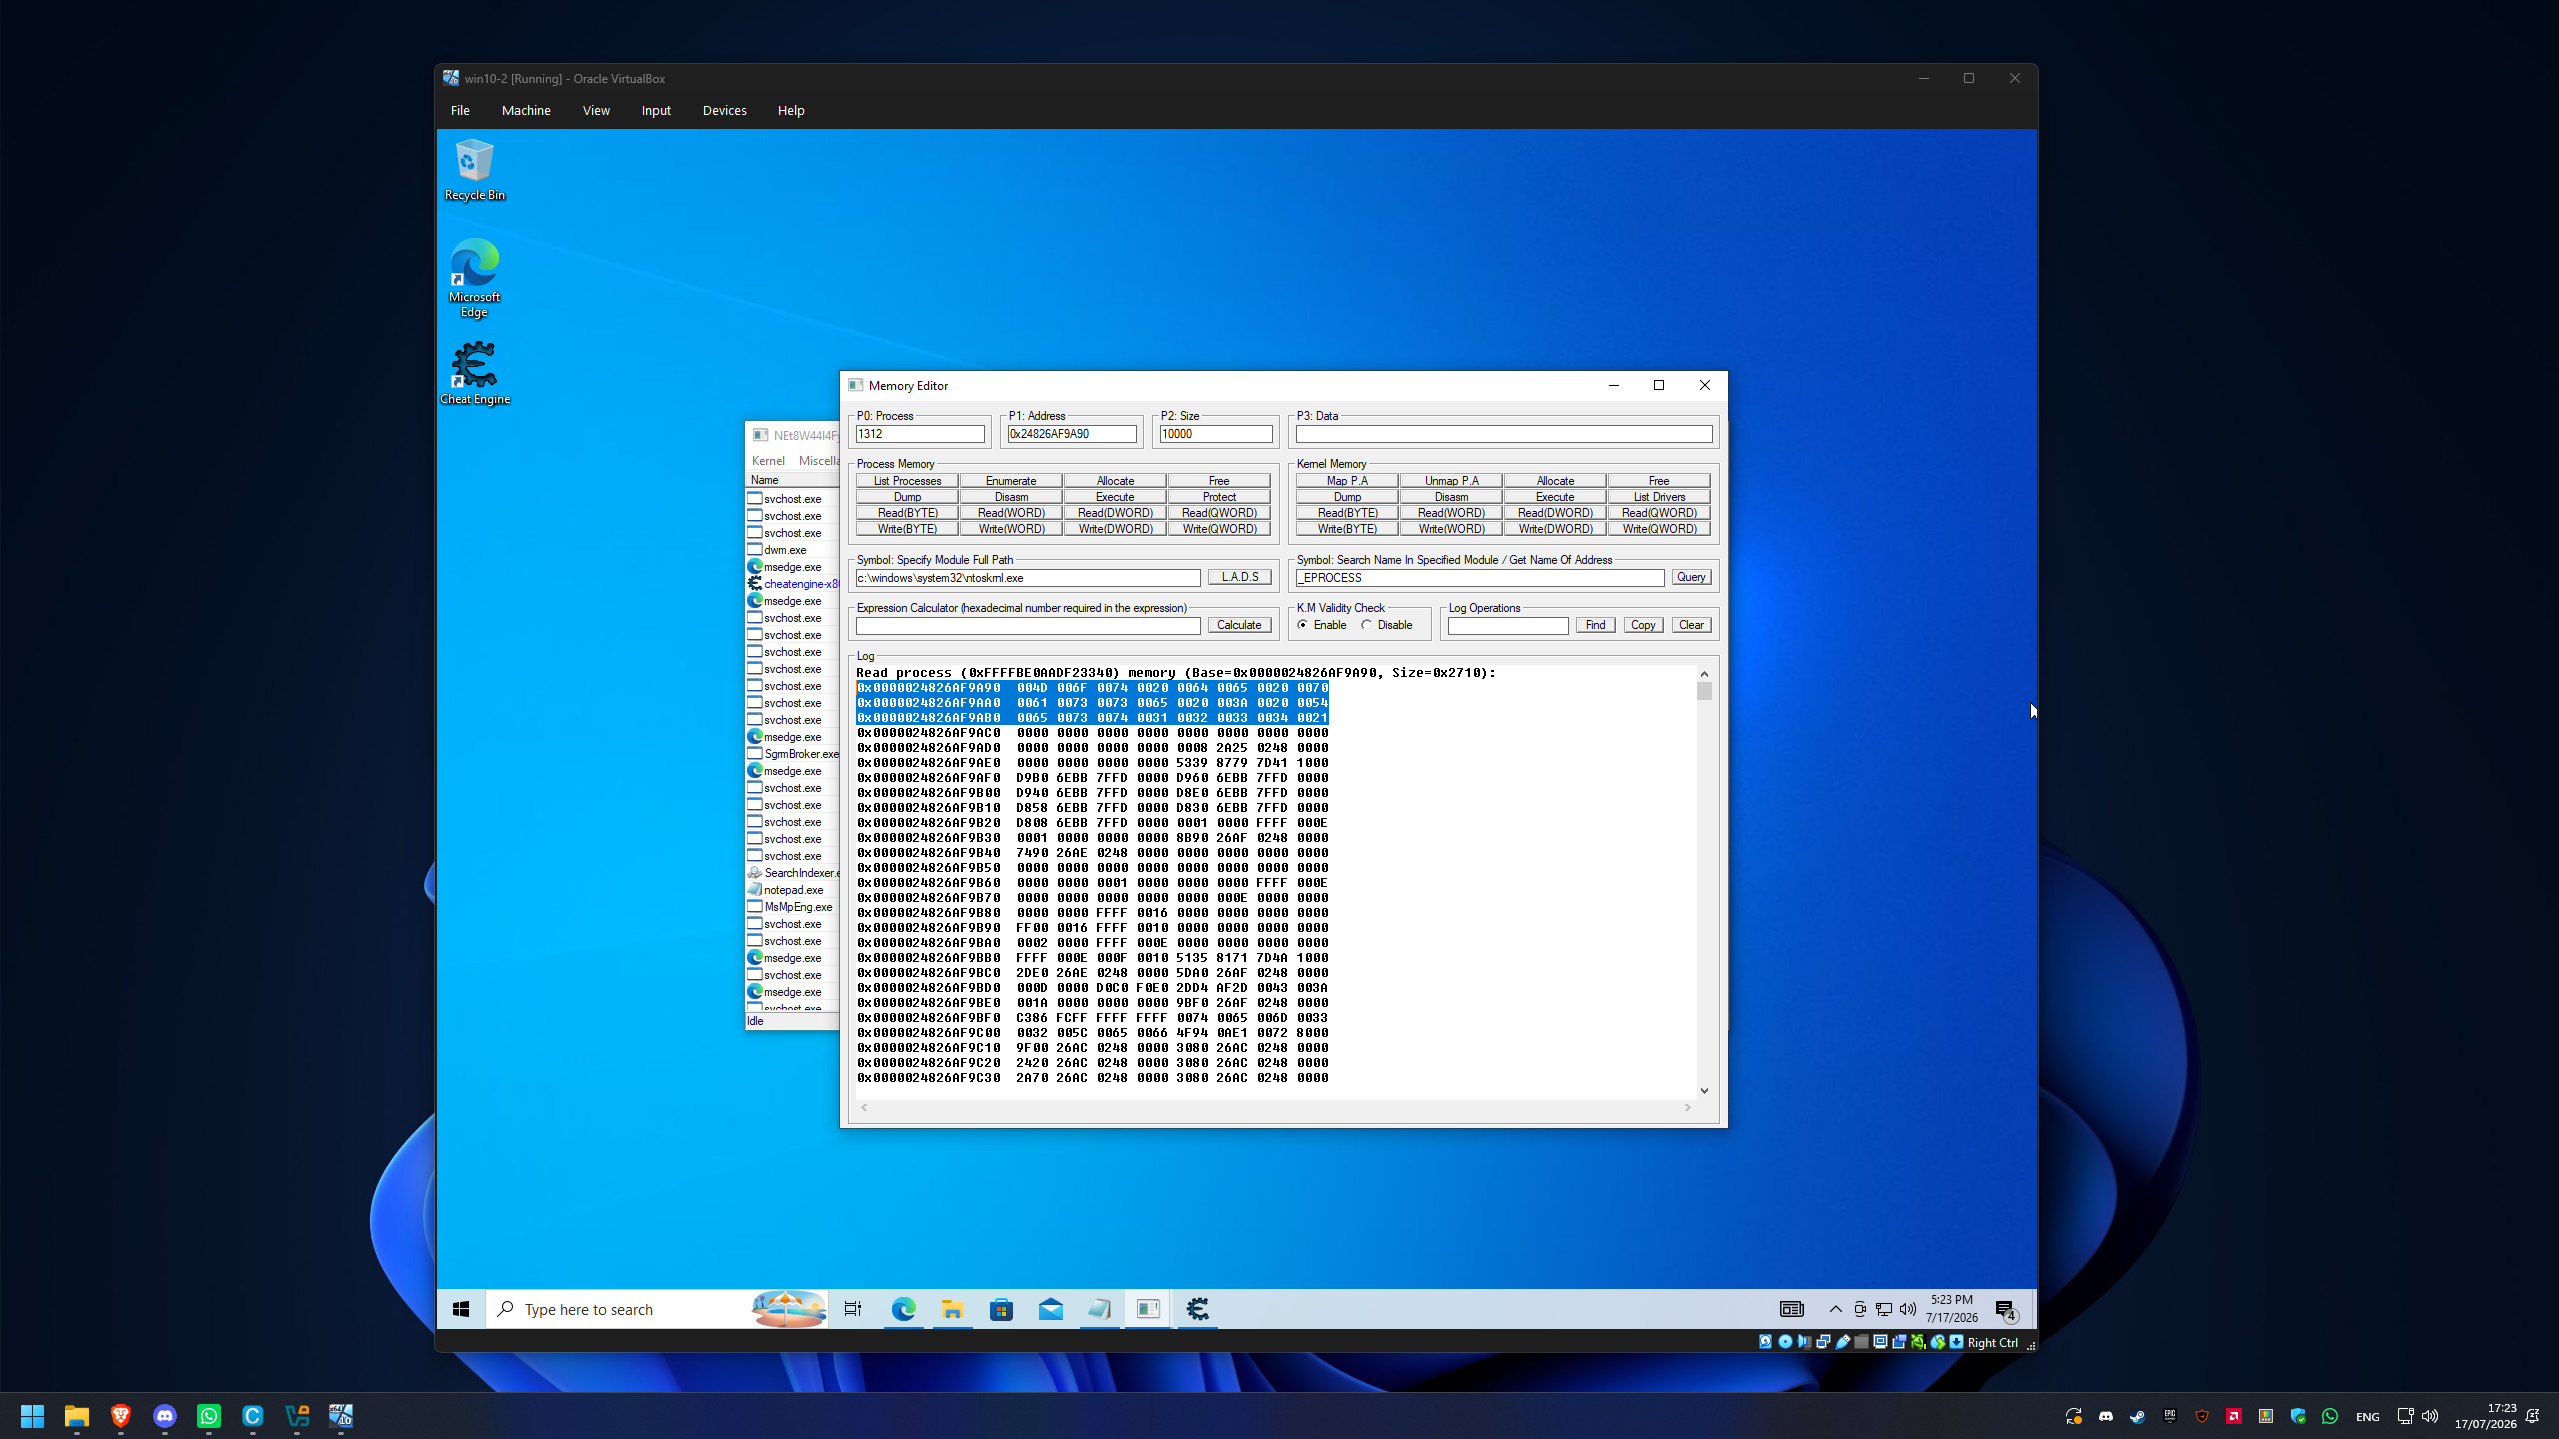
\includegraphics[height=4cm]{../images/chap02/15.png}
	\end{center}
\end{frame}

% SLIDE
\beamerdefaultoverlayspecification{}
\begin{frame}
	\frametitle{Problem}
	\visible<1->{
			If detection at this privilege level is both:
			\begin{itemize}
				\item Intrusive: capable of reading anything on the machine
				\item Bypassable: outpaced by DMA cheats
			\end{itemize}
		}
	\vspace{1cm}
	\visible<2->{
			\bf Is there a way to detect cheating without it?
		}
\end{frame}
\beamerdefaultoverlayspecification{<+->}
